\documentclass[12pt, letterpaper]{article}

\usepackage[utf8]{inputenc}
\usepackage{hyperref}
\usepackage{epsfig, url}
\usepackage{epstopdf}
\usepackage{graphicx}
\usepackage{datetime}
\usepackage{multirow}
\usepackage{rotating}


%\usepackage{wrapfig}
%\usepackage{amsmath}
\usepackage{amssymb}
\usepackage{geometry} 
\geometry{a4paper}              

\usepackage{titling}

\setlength{\evensidemargin}{0in}
\setlength{\oddsidemargin}{0in}
\setlength{\textwidth}{6.5in}
\setlength{\textheight}{9.0in}
\setlength{\topmargin}{0in}
\setlength{\headheight}{0in}
\setlength{\headsep}{0in}
\setlength{\itemsep}{-\parsep}



\begin{document}
\title{\large Course CS549 Assignment 1\\[0.5cm]
        \bf\Large Implementation of the DES algorithm}
\author{\large Sreeparna Das (226101004)\\
\\
        \large Vishal Kumar (226101005)\\
\\
        \large Akash Lal Dutta (226101001)}
        
\date{February 19, 2023}
\makeatletter
    \begin{titlepage}
        \begin{center}
        \vbox{}\vspace{5cm}
            {\@title }\\[3cm] 
            {\@author}\\
            %{Instructor: \bf instructor name}\\
            \vfill 
\includegraphics[scale=0.2]{images/IITG_logo.png}\\[0.4cm]
            {\@date}
        \end{center}
    \end{titlepage}
\makeatother
%\thispagestyle{empty}




\newpage
\tableofcontents
\newpage
\listoftables
\listoffigures
\newpage

\addcontentsline{toc}{section}{\nameref{intro}}
\section*{The DES Algorithm : Introduction}
\label{intro}
The Data Encryption Standard (DES) algorithm is a symmetric-key block cipher used for encrypting and decrypting digital data. It takes a 64-bit block of plain-text and a 64-bit key as inputs, and produces a 64-bit block of cipher-text as output.\\
\\
The algorithm consists of 16 rounds, each using a different 48-bit sub-key generated from the original 64-bit key. In each round, the 64-bit plain-text is first split into two 32-bit halves, and then a function is applied to one half using the sub-key. The result is XOR-ed with the other half, and the two halves are swapped before moving on to the next round.\\
\\
The function applied in each round includes an expansion permutation, which expands the 32-bit input into a 48-bit value, and a substitution step, which replaces the 48-bit value with a different 32-bit value using a set of predefined substitution boxes. The output of the substitution step is then subjected to a permutation, known as the P-box permutation, before being XOR-ed with the other half.\\
\\
After all 16 rounds have been completed, the final 64-bit output is subjected to a final permutation, which shuffles the bits according to a predetermined pattern to produce the final cipher-text.\\
\\
The same algorithm and key are used for encryption and decryption, the only difference being the order in which the sub-keys are used in the rounds.


\section{Structure of a key in DES Algorithm}
\label{Hand-cal}
The key in the DES algorithm is a 64-bit value used to encrypt and decrypt data. The key undergoes transformation and permutation during the key generation process to create 16 sub-keys, one for each of the 16 rounds of the DES algorithm. Each sub-key is a 48-bit value used to modify the plain-text during each round of encryption or decryption. The sub-keys are generated from the original 64-bit key through permutation, shifting, and compression.\\
\\
The DES algorithm uses a technique known as the Feistel network, which means that the data is divided into two halves, left and right, and each half undergoes a series of modifications using the sub-keys. The left and right halves are swapped after each round, and the modifications are repeated. The sub-keys are generated using a combination of the original key and the results of the previous round of modifications.\\
\\
The key plays a crucial role in the DES algorithm, as it determines the encryption and decryption process. To ensure the security of the data, it is important to choose a strong and unique key. However, the DES algorithm has since been replaced by more secure encryption algorithms such as AES.

\begin{figure}[hbt!]
    \centering
    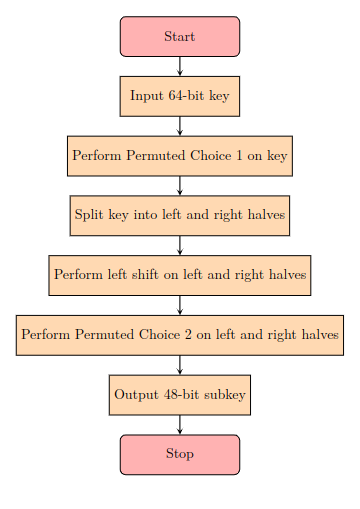
\includegraphics[scale=0.6, angle=0]{images/Screenshot from 2023-02-18 21-07-04.png}
    \caption{Flowchart of the Key Generation}
    \label{fig:crazy}
\end{figure}


\section{Implementation of DES Algorithm}

\begin{enumerate}
\item \textbf{Key Generation:} The 64-bit key can be input as a string of hexadecimal characters and converted to a binary string. The key generation algorithm can then be implemented to produce 16 round sub-keys of 48-bits each.

\item \textbf{Initial Permutation:} The 64-bit plain-text can also be input as a string of hexadecimal characters and converted to a binary string. The initial permutation algorithm can then be implemented to rearrange the bits according to a fixed permutation table.

\item \textbf{Round Function:} The 64-bit plain-text can be divided into 32-bit blocks (LPT and RPT) using slicing. Each round can then consist of the following steps:

\begin{enumerate}
\item Expansion Permutation: The RPT block can be expanded from 32-bits to 48-bits using a fixed permutation table.

\item Subkey Mixing: The expanded RPT block can be XORed with the corresponding 48-bit subkey for that round. The subkeys can be generated by selecting the appropriate 48-bits from the round subkeys produced in the key generation step.

\item S-Box Substitution: The resulting 48-bit block can then be divided into 8 6-bit blocks, each of which is substituted using a fixed S-box. The S-boxes can be implemented using lookup tables.

\item Permutation: The resulting 32-bit block can be rearranged using a fixed permutation table.

\item LPT and RPT Update: The resulting 32-bit block can be XORed with the LPT block, and the RPT block becomes the new LPT block.
\end{enumerate}

\item \textbf{Final Permutation:} After the 16 rounds are completed, the LPT and RPT can be swapped and then subjected to a final permutation using a fixed permutation table to produce the 64-bit ciphertext.
\end{enumerate}
The output of each step in the DES algorithm, including the LPT and RPT after each round and the ciphertext, can be printed or stored in variables for further analysis.

\begin{figure}[hbt!]
    \centering
    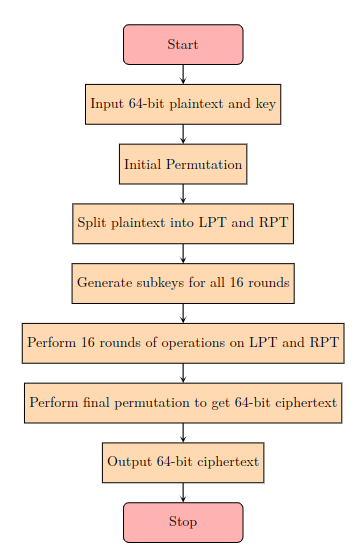
\includegraphics[scale=0.6, angle=0]{images/Screenshot from 2023-02-18 21-05-04.png}
    \caption{DES Algorithm}
    \label{fig:crazy}
\end{figure}



        
\section{Assignment Overview}

In our case, the 64-bit plain-text is formed using the last eight digits of two students' roll numbers, and the 64-bit key is formed using the last eight digits of two other students' roll numbers. The output of each step in the DES algorithm, including the \textbf{LPT} and \textbf{RPT} after each round and the cipher-text, should be documented for the given input.

    \subsection{Results to be produced}

    \begin{enumerate}
  \item Initial permutation (mention LPT and RPT)
  \item For all 16 rounds:
  \begin{enumerate}
    \item Expansion permutation
    \item Sub-key used in the round
    \item LPT and RPT after the round
  \end{enumerate}
  \item Final permutation (mention Cipher-text)
\end{enumerate}

\subsection{Given Data}

\begin{table}[h]
    \centering
    \begin{tabular}{|c|c|}
        \hline
        \textbf{Student Name} & \textbf{Roll Number} \\
        \hline
        Sreeparna Das & 26101004 \\
        \hline
        Vishal Kumar & 26101005 \\
        \hline
        Akash Lal Dutta & 26101001 \\
        \hline
        Dummy Name & 26101006 \\
        \hline
    \end{tabular}
    \caption{Student Information}
    \label{tab:student-info}
\end{table} \\

\underline{\textbf{Roll numbers in binary}}\\
\\
Student S1 roll number = 0010 0110 0001 0000 0001 0000 0000 0100\\
\\
Student S2 roll number = 0010 0110 0001 0000 0001 0000 0000 1001\\
\\
Student S3 roll number = 0010 0110 0001 0000 0001 0000 0000 0001\\
\\
Student S4 roll number = 0010 0110 0001 0000 0001 0000 0000 0110\\

\underline{\textbf{For student S1}} : \\
\\

\begin{table}[h]
    \centering
    \begin{tabular}{|c|c|}
        \hline
          Plain Text & Key \\
        \hline
        \textbf{S1 S2} & \textbf{S3 S4} \\
        \hline
    \end{tabular}
    \caption{Plain-Text and Key for S1}
    \label{tab:text-key}
\end{table}

\subsection{Encryption}

\underline{\textbf{Initial Permutation}} \\
\\
\begin{table}[h]
    \centering
    \begin{tabular}{|c|c|}
        \hline
        LPT & RPT \\
        \hline
        0000 0000 0110 0110 1001 1001 1000 0000 & 0000 0000 0001 0001 0000 0000 0001 0001  \\
        \hline
    \end{tabular}
    \caption{LPT and RPT Values}
    \label{tab:lpt-rpt}
\end{table}


\begin{table}[ht]
  \centering
  \label{tab:sample-table}
  \begin{tabular}{|c|c|c|}
    \hline
    Round & LPT & RPT  \\
    \hline
    1 & 0000 0000 0001 0001 0000 0000 0001 0001  & 0101 0101 0010 1110 0100 0100 0001 1101  \\
        \hline
    2 & 0101 0101 0010 1110 0100 0100 0001 1101

 & 0010 1100 1010 0000 0001 0011 1010 0011

  \\
         \hline
    3 & 0010 1100 1010 0000 0001 0011 1010 0011 & 1000 1010 1010 1000 0100 1100 0100 1000  \\
         \hline
    4 & 1000 1010 1010 1000 0100 1100 0100 1000 & 0111 0011 0001 1101 1011 0101 0100 0000  \\
         \hline
    5 & 0111 0011 0001 1101 1011 0101 0101 0000 & 1111 1010 0110 0001 0000 1000 0000 1000  \\
        \hline
    6 & 1111 1010 0110 0001 0000 1000 0000 1000 & 0011 0101 0101 1100 0110 0010 1100 1111  \\
         \hline
    7 & 0011 0101 0101 1100 0110 0010 1100 1111 & 0010 1011 0111 1100 0001 1100 1011 0110

  \\
         \hline
    8 & 0010 1011 0111 1100 0001 1100 1011 0110

 & 0010 1110 0010 1100 1110 0100 1100 1101

  \\
         \hline
    9 & 0010 1110 0010 1100 1110 0100 1100 1101

 & 1010 0010 0100 1001 0111 0110 0000 0010

  \\
         \hline
    10 & 1010 0010 0100 1001 0111 0110 0000 0010

 & 1100 0010 0011 0100 0101 1110 1010 1001

  \\
         \hline
    11 & 1100 0010 0011 0100 0101 1110 1010 1001

 & 0010 0111 0110 0101 0110 0011 1000 1010

  \\
         \hline
    12 & 0010 0111 0110 0101 0110 0011 1000 1010

 & 0101 1101 0010 0110 1110 1000 1111 1110

  \\
         \hline
    13 & 0101 1101 0010 0110 1110 1000 1111 1110

 & 0011 1001 1110 0000 1100 0000 0000 0010  \\
         \hline
    14 & 0011 1001 1110 0000 1100 0000 0000 0010 & 0001 0111 0001 0110 0100 1110 1110 0001

  \\
         \hline
    15 & 0001 0111 0001 0110 0100 1110 1110 0001

 & 1101 1011 1111 0111 1100 0000 1100 0100

  \\
         \hline
    16 & 1101 1011 1111 0111 1100 0000 1100 0100

 & 1101 1011 1111 0111 1100 0000 1100 0100

  \\
    \hline
  \end{tabular}
    \caption{Operations for all 16 Rounds}

    

\end{table}

\begin{table}[h]
    \centering
    \begin{tabular}{|c|}
        \hline
          Binary Key \\
        \hline
        0010 0110 0001 0000 0001 0000 0000 0001 0010 0110 0001 0000 0001 0000 0000 0110  \\
        \hline
    \end{tabular}
    \caption{Key for S1}
    \label{tab:text-key}
\end{table}

\begin{table}[h]
    \centering
    \begin{tabular}{|c|}
        \hline
          Sub-Key\\
        \hline
        0000 0000 0000 0000 0001 0001 0110 1001 0001 1001 0001 0000 0000 0110 \\
        \hline
    \end{tabular}
    \caption{PC-1 Key for S1}
    \label{tab:text-key}
\end{table}

\begin{table}[h]
    \centering
    \begin{tabular}{|c|c|}
        \hline
        \textbf{Round} & \textbf{Sub-Key} \\
        \hline
        1 & 0000 0000 0000 1100 1000 0000 0010 0000 0000 0011 0100 0100
 \\
        \hline
        2 & 0001 0000 0000 0000 0000 0000 0100 0110 0000 0000 1101 0000
 \\
        \hline
        3 & 0000 0000 0000 1000 0010 0100 0000 0001 1010 0001 0100 1101
 \\
        \hline
        4 & 1000 0000 0010 0000 0000 0100 0010 0010 1001 0100 1000 0000
 \\
        \hline
        5 & 0000 0000 0000 0110 0010 0000 0100 1000 0000 0101 0010 0111
 \\
        \hline 
        6 & 1100 0000 0001 0000 0010 0000 0000 1110 0100 1000 1000 1000
 \\
        \hline
        7 & 1000 0000 1000 0010 0100 0000 0100 0000 0101 0001 0101 0001
 \\
        \hline
        8 & 0000 0000 0101 0010 0000 0010 1000 0011 1000 0000 0010 1000
 \\
        \hline
        9 & 0010 0100 0000 0010 0000 0000 0000 0001 0100 0110 0101 1010
 \\
        \hline
        10 & 0000 0010 0001 0000 0001 0000 0001 1101 1001 0000 0000 0000
 \\
        \hline
        11 & 0000 1100 0000 0000 0101 0000 1000 0000 0100 0100 0110 0100
 \\
        \hline
        12 & 0000 0110 0100 0000 0000 1000 0000 1000 1010 1010 1000 0100 \\
        \hline
        13 & 0000 1010 0000 0001 0000 0000 1011 0000 0100 0100 1001 0001 \\
        \hline
        14 & 0000 1000 0000 1000 0000 1001 0000 1011 0000 0010 0000 0011
 \\
        \hline
        15 &  0000 0001 0010 0000 0000 1000 1001 0110 0110 0001 0000 0000 \\
        \hline
        16 & 0001 0000 0000 0000 1000 1100 0001 0101 0000 1000 0000 0111 \\
        \hline

    \end{tabular}
    \caption{Sub-Key Generated Table}
    \label{tab:student-info}
\end{table}

\begin{table}[h]
    \centering
    \begin{tabular}{|c|}
        \hline
          Cipher Text \\
        \hline
           1111 0101 1111 0100 0110 0111 1001 0001 1111 0111 0001 1011 1110 1111 1011
  \\
        \hline
    \end{tabular}
    \caption{Cipher Text Generated}
    \label{tab:text-key}
\end{table}

\begin{table}[h]
    \centering
    \begin{tabular}{|c|c|}
        \hline
        LPT & RPT \\
        \hline
         1011 0111 1111 1011 0101 0111 1011 1101 & 1101 1011 1111 0111 1100 0000 1100 0100  \\
        \hline
    \end{tabular}
    \caption{LPT and RPT Values}
    \label{tab:lpt-rpt}
\end{table}


\begin{table}[ht]
  \centering
  \label{tab:sample-table}
  \begin{tabular}{|c|c|c|}
    \hline
    Round & LPT & RPT  \\
    \hline
    1 &  1101 1011 1111 0111 1100 0000 1100 0100  & 0001 0111 0001 0110 0100 1110 1110 0001
  \\
        \hline
    2 & 0001 0111 0001 0110 0100 1110 1110 0001

 & 0011 1001 1110 0000 1100 0000 0000 0010


  \\
         \hline
    3 &  0011 1001 1110 0000 1100 0000 0000 0010 & 0101 1101 0010 0110 1110 1000 1111 1110
  \\
         \hline
    4 &  0101 1101 0010 0110 1110 1000 1111 1110 & 0010 0111 0110 0101 0110 0011  1000 1010
  \\
         \hline
    5 &  0010 0111 0110 0101 0110 0011  1000 1010 & 1100 0010 0011 0100 0101 1110 1010 1001
  \\
        \hline
    6 & 1100 0010 0011 0100 0101 1110 1010 1001 & 1010 0010 0100 1001 0111 0110 0000 0010
  \\
         \hline
    7 &  1010 0010 0100 1001 0111 0110 0000 0010 & 0010 1110 0010 1100 1110 0100 1100 1101

  \\
         \hline
    8 & 0010 1110 0010 1100 1110 0100 1100 1101

 & 0010 1011 0111 1100 0001 1100 1011 0110

  \\
         \hline
    9 & 0010 1011 0111 1100 0001 1100 1011 0110

 & 0011 0101 0101 1100 0110 0010 1100 1111


  \\
         \hline
    10 & 0011 0101 0101 1100 0110 0010 1100 1111

 & 1111 1010 0110 0001 0000 1000 0000 1000

  \\
         \hline
    11 & 1111 1010 0110 0001 0000 1000 0000 1000

 & 0111 0011 0001 1011 0101 0100 0101 0000

  \\
         \hline
    12 & 0111 0011 0001 1011 0101 0100 0101 0000

 & 1000 0110 1010 1000 0100 1100 0100 1000

  \\
         \hline
    13 & 1000 0110 1010 1000 0100 1100 0100 1000

 & 0010 1100 1010 0000 0001 0011 1010 0011 \\
         \hline
    14 & 0010 1100 1010 0000 0001 0011 1010 0011 & 0101 0101 0010 1110 0100 0100 0001 1101

  \\
         \hline
    15 & 0101 0101 0010 1110 0100 0100 0001 1101

 & 0000 0000 0001 0001 0000 0000 0001 0001

  \\
         \hline
    16 &   0000 0000 0110 0110 1001 1001 1000 0000

 & 0000 0000 0001 0001 0000 0000 0001 0001

  \\
    \hline
  \end{tabular}
    \caption{Operations for all 16 Rounds of Decryption}

    

\end{table}

\begin{table}[h]
    \centering
    \begin{tabular}{|c|}
        \hline
          Binary Key \\
        \hline
        0010 0110 0001 0000 0001 0000 0000 0001 0010 0110 0001 0000 0001 0000 0000 0110  \\
        \hline
    \end{tabular}
    \caption{Key for S1}
    \label{tab:text-key}
\end{table}

\begin{table}[h]
    \centering
    \begin{tabular}{|c|}
        \hline
          Sub-Key\\
        \hline
        0000 0000 0000 0000 0001 0001 0110 1001 0001 1001 0001 0000 0000 0110 \\
        \hline
    \end{tabular}
    \caption{PC-1 Key for S1}
    \label{tab:text-key}
\end{table}

\begin{table}[h]
    \centering
    \begin{tabular}{|c|c|}
        \hline
        \textbf{Round} & \textbf{Sub-Key} \\
        \hline
        1 & 0001 0000 0000 0000 1000 1100 0001 0101 0000 1000 0000 0111
 \\
        \hline
        2 &  0000 0001 0010 0000 0000 1000 1001 0110 0110 0001 0000 0000
 \\
        \hline
        3 & 0000 1000 0000 1000 0000 1001 0000 1011 0000 0010 0000 0011
 \\
        \hline
        4 & 0000 1010 0000 0001 0000 0000 1011 0000 0100 0100 1001 0001
 \\
        \hline
        5 & 0000 0110 0100 0000 0000 1000 0000 1000 1010 1010 1000 0100
 \\
        \hline 
        6 & 0000 1100 0000 0000 0101 0000 1000 0000 0100 0100 0110 0100
 \\
        \hline
        7 & 0000 0010 0001 0000 0001 0000 0001 1101 1001 0000 0000 0000
 \\
        \hline
        8 &  0010 0100 0000 0010 0000 0000 0000 0001 0100 0110 0101 1010
 \\
        \hline
        9 & 0000 0000 0101 0010 0000 0010 1000 0011 1000 0000 0010 1000
 \\
        \hline
        10 & 1000 0000 1000 0010 0100 0000 0100 0000 0101 0001 0101 0001
 \\
        \hline
        11 & 1100 0000 0001 0000 0010 0000 0000 1110 0100 1000 1000 1000
 \\
        \hline
        12 & 0000 0000 0000 0110 0010 0000 0100 1000 0000 0101 0010 0111 \\
        \hline
        13 &  1000 0000 0010 0000 0000 0100 0010 0010 1001 0100 1000 0000 \\
        \hline
        14 & 0000 0000 0000 1000 0010 0100 0000 0001 1010 0001 0100 1101
 \\
        \hline
        15 &   0001 0000 0000 0000 0000 0000 0100 0110 0000 0000 1101 0000 \\
        \hline
        16 &  0000 0000 0000 1100 1000 0000 0010 0000 0000 0011 0100 0100 \\
        \hline

    \end{tabular}
    \caption{Sub-Key Generated Table for Decryption}
    \label{tab:student-info}
\end{table}

\begin{table}[h]
    \centering
    \begin{tabular}{|c|}
        \hline
          Plain Text \\
        \hline
           010 0110 0001 0000 0001 0000 0000 0100 010 0110 0001 0000 0001 0000 0000 1001
  \\
        \hline
    \end{tabular}
    \caption{Plain Text Generated}
    \label{tab:text-key}
\end{table}





\end{document}










\newpage
\bibliographystyle{ieeetr}
\bibliography{ref}

\end{document}
